

\section{Detector Apparatus}
\label{sec:cmsexperiment:detector}



% overview
The CMS \cite{exhep:cms:Chatrchyan:2008aa} detector is a general-purpose apparatus located about 100~m underground at Point~5 of the LHC. It is close to the French village of Cessy, between Lake Geneva and the Jura mountains. As a general-purpose detector, the CMS detector is designed to observe new physics phenomena that the LHC might reveal \cite{cms:tdr2:Ball:2007zza}. At the designed LHC luminosity of $10^{34}$~\percms, about 20 inelastic collisions on average are superimposed on the event of interest every collision of bunch crossings, leading to a large flux of particles originating from the collision point to enter the detector every 25 ns. To discern them and trigger the interested events within 25 ns latency over the LHC run period until 2035, the CMS detector is designed to be highly-segmented, radiation-hard and with good timing resolution \cite{exhep:cms:Chatrchyan:2008aa}.

\begin{figure}[ht]
    \centering
    \includegraphics[width=0.98\textwidth]{chapters/CMSExperiment/sectionDetector/figures/cmsDetector.png}
    \caption{The layout of the CMS detector \cite{cms:detectorOverview}.}
    \label{fig:cmsexperiment:detector:detectorOverview}
\end{figure}

% overview of structure
The apparatus layout of the CMS detector is shown in Figure~\ref{fig:cmsexperiment:detector:detectorOverview} \cite{cms:detectorOverview}. The central feature of the CMS apparatus is a superconducting solenoid of 6~m internal diameter, providing a magnetic field of 3.8~T. Within the superconducting solenoid volume are a silicon pixel and strip tracker, a lead tungstate crystal electromagnetic calorimeter, and a brass and scintillator hadron calorimeter, each composed of a barrel and two endcap sections. Muons are measured in gas-ionization detectors embedded in the steel flux-return yoke outside the solenoid. Additional forward calorimetry complements the coverage of the barrel and endcap detectors. More details of these sub-systems are discussed in this section. 

% To achieve the physics goal in the LHC environment, the design of each CMS sub-detectors are driven by the following performance requirement.

% \begin{itemize}
%     \item Magnets and Muon chamber: Good muon identification, energy resolution, charge determination.
%     \item Pixel and Tracker: Good charge hadron track reconstruction efficiency. Good displaced vertex tagging for $b$, $\tau$ identification.
%     \item ECAL: Good electromagnetic energy resolution. $\pi^0$ rejection. Efficient photon and lepton isolation at high luminosities.
%     \item HCAL: Good missing-transverse-energy and dijet-mass resolution
% \end{itemize}



\subsection{Magnet}
% overview
The CMS superconducting magnet \cite{cms:magnetTdr:Acquistapace:1997fm} is used to provide bending to the charged particles as they traverse, which is crucial to both particle identification and momentum measurement. The internal magnetic field is 4~Tesla with 2.6~GJ stored energy generated by a superconducting solenoid. The solenoid is 12.5~m in length, 6.3~m in diameter, and 200~tons in weight, consist of 41.7~MA-turn of wire. The radiation thickness of the solenoid is 4.9~$\chi_0$, which further prevents hadrons from entering the muon system. The solenoid is surrounded and mechanically supported by the iron return yoke, which directs the outer magnetic field in the muon system. The yoke, consisting of 5 barrel wheels and two endcaps, has an outer diameter of 14~m and a weight of 10000~ton. Both barrel and endcap return yoke have three iron layers with thicknesses of 300/630/630~mm and 250/600/600~mm, respectively.


\subsection{Inner Tracking System}
% overview
The inner tracking system \cite{cms:trackerTdr:CMS:1997tlf} is used to measure the trajectories of charged particles. It consists of two major parts: pixel detector and Silicon strip tracker, and covers the region with $|\eta|<2.5$. The layout of the inner tracking system is shown in Figure~\ref{fig:cmsexperiment:detector:tracker}.  The material thickness of the tracking system is shown in Figure~\ref{fig:cmsexperiment:detector:trackerMaterial}.


\begin{figure}[ht]
    \centering
    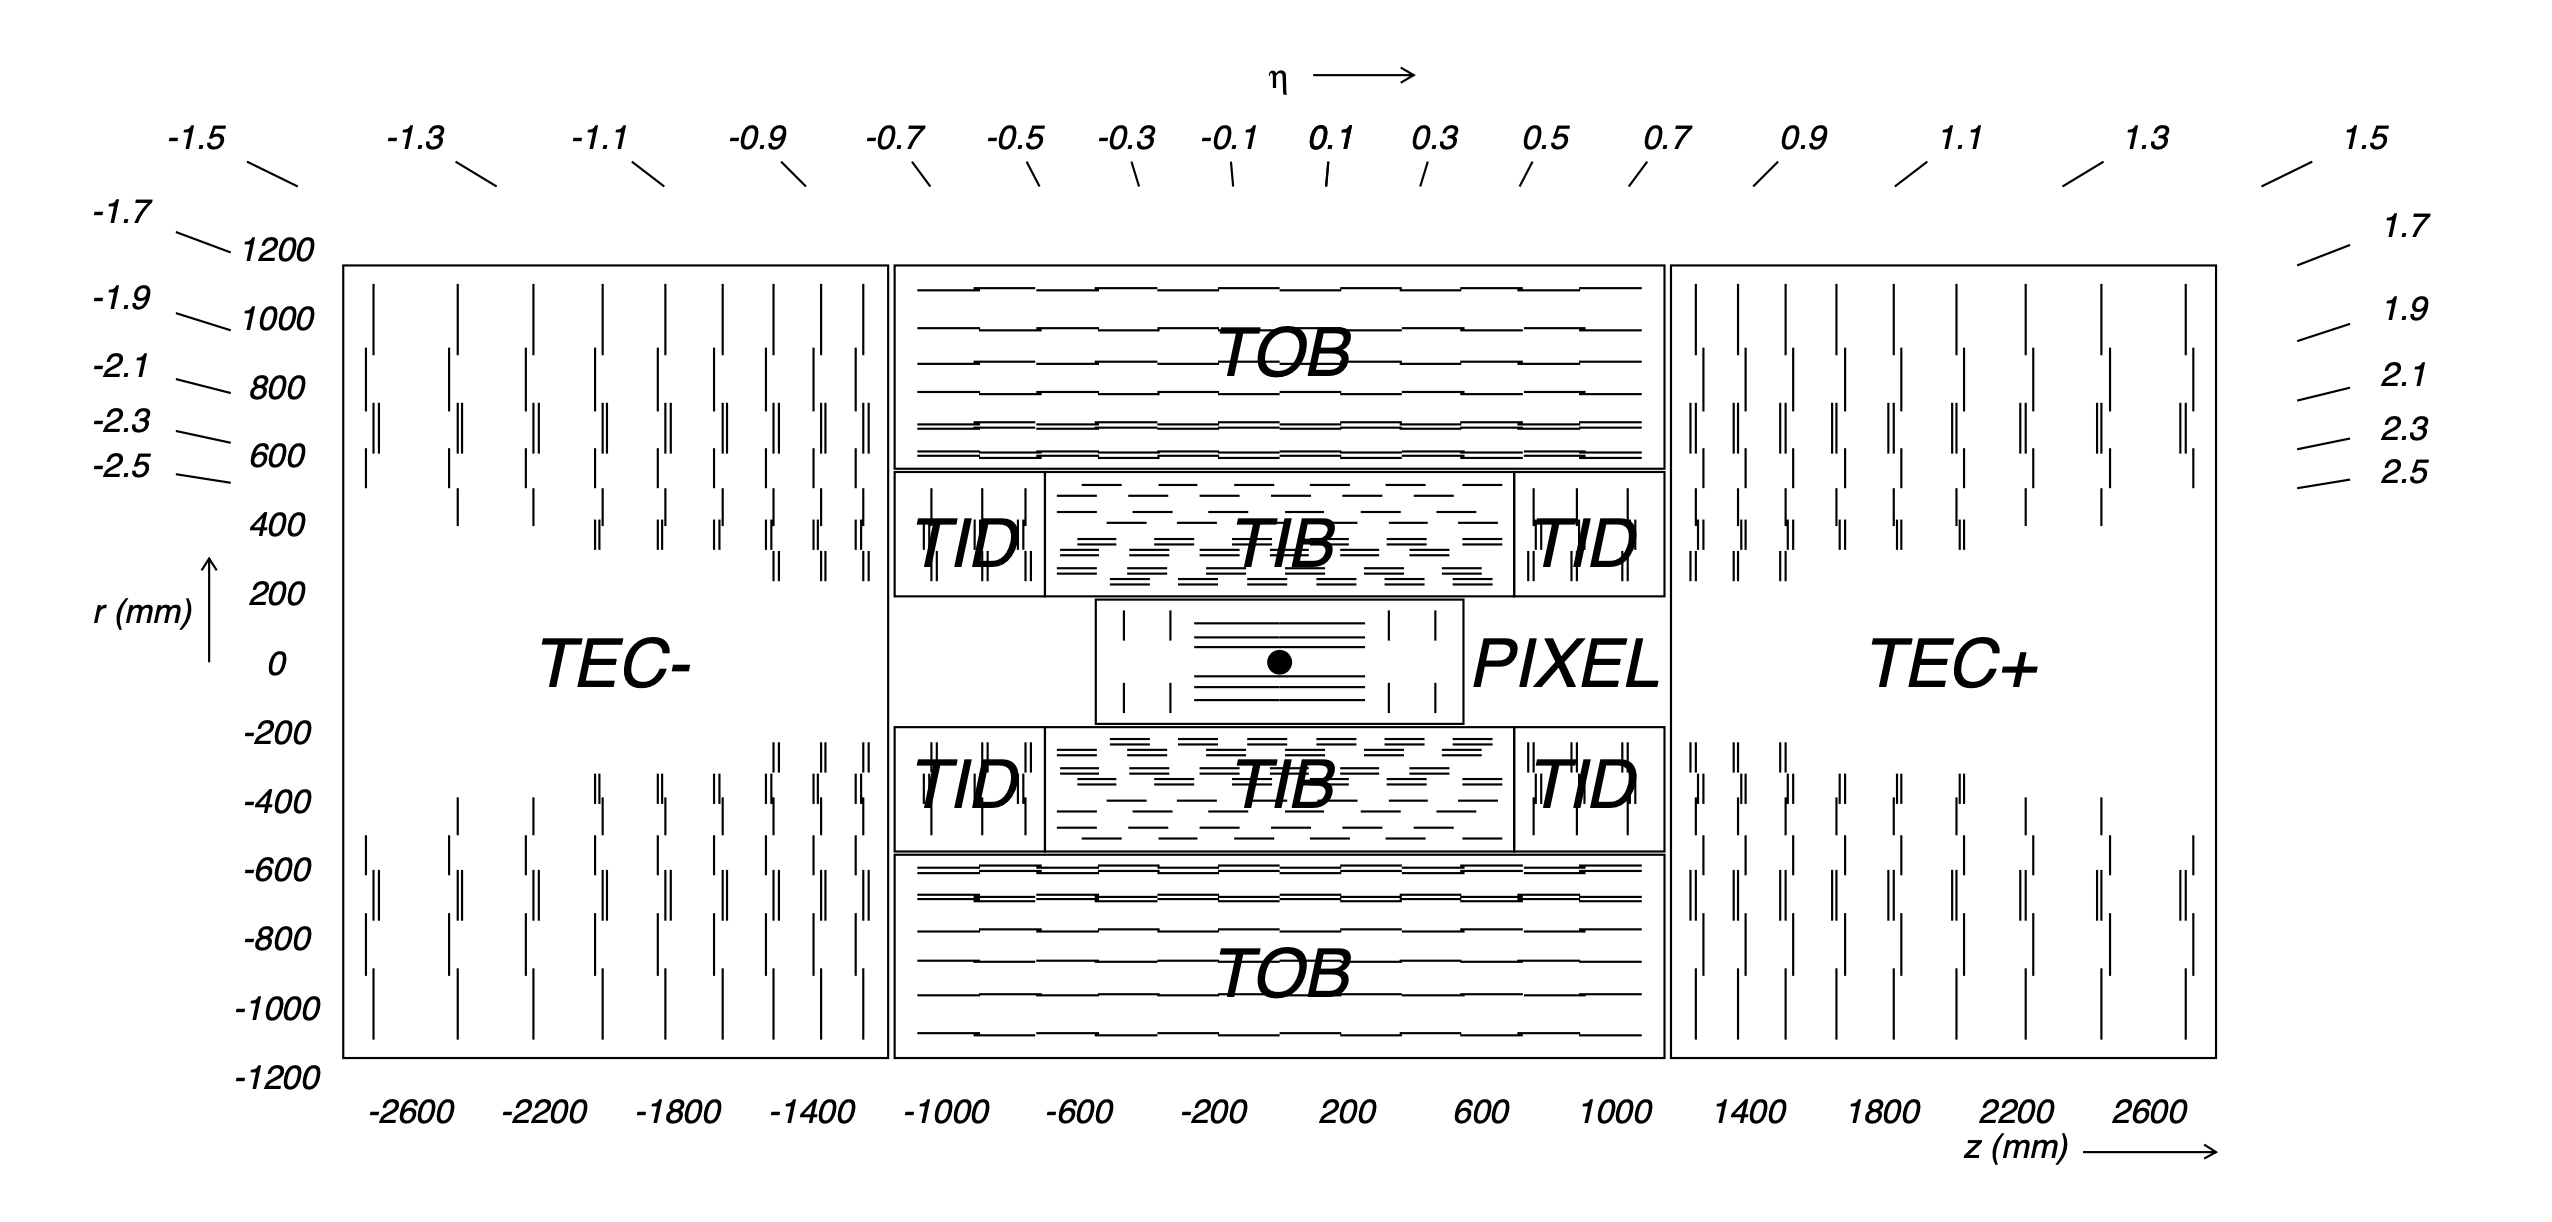
\includegraphics[width=0.98\textwidth]{chapters/CMSExperiment/sectionDetector/figures/tracker.png}
    \caption{The layout of the CMS inner tracking system \cite{exhep:cms:Chatrchyan:2008aa}. It is consist of pixel detector and silicon strip tracker (TIB/TID, TOB, TEC), covering regions with $|\eta|<2.5$. }
    \label{fig:cmsexperiment:detector:tracker}
\end{figure}


\begin{figure}[ht]
    \centering
    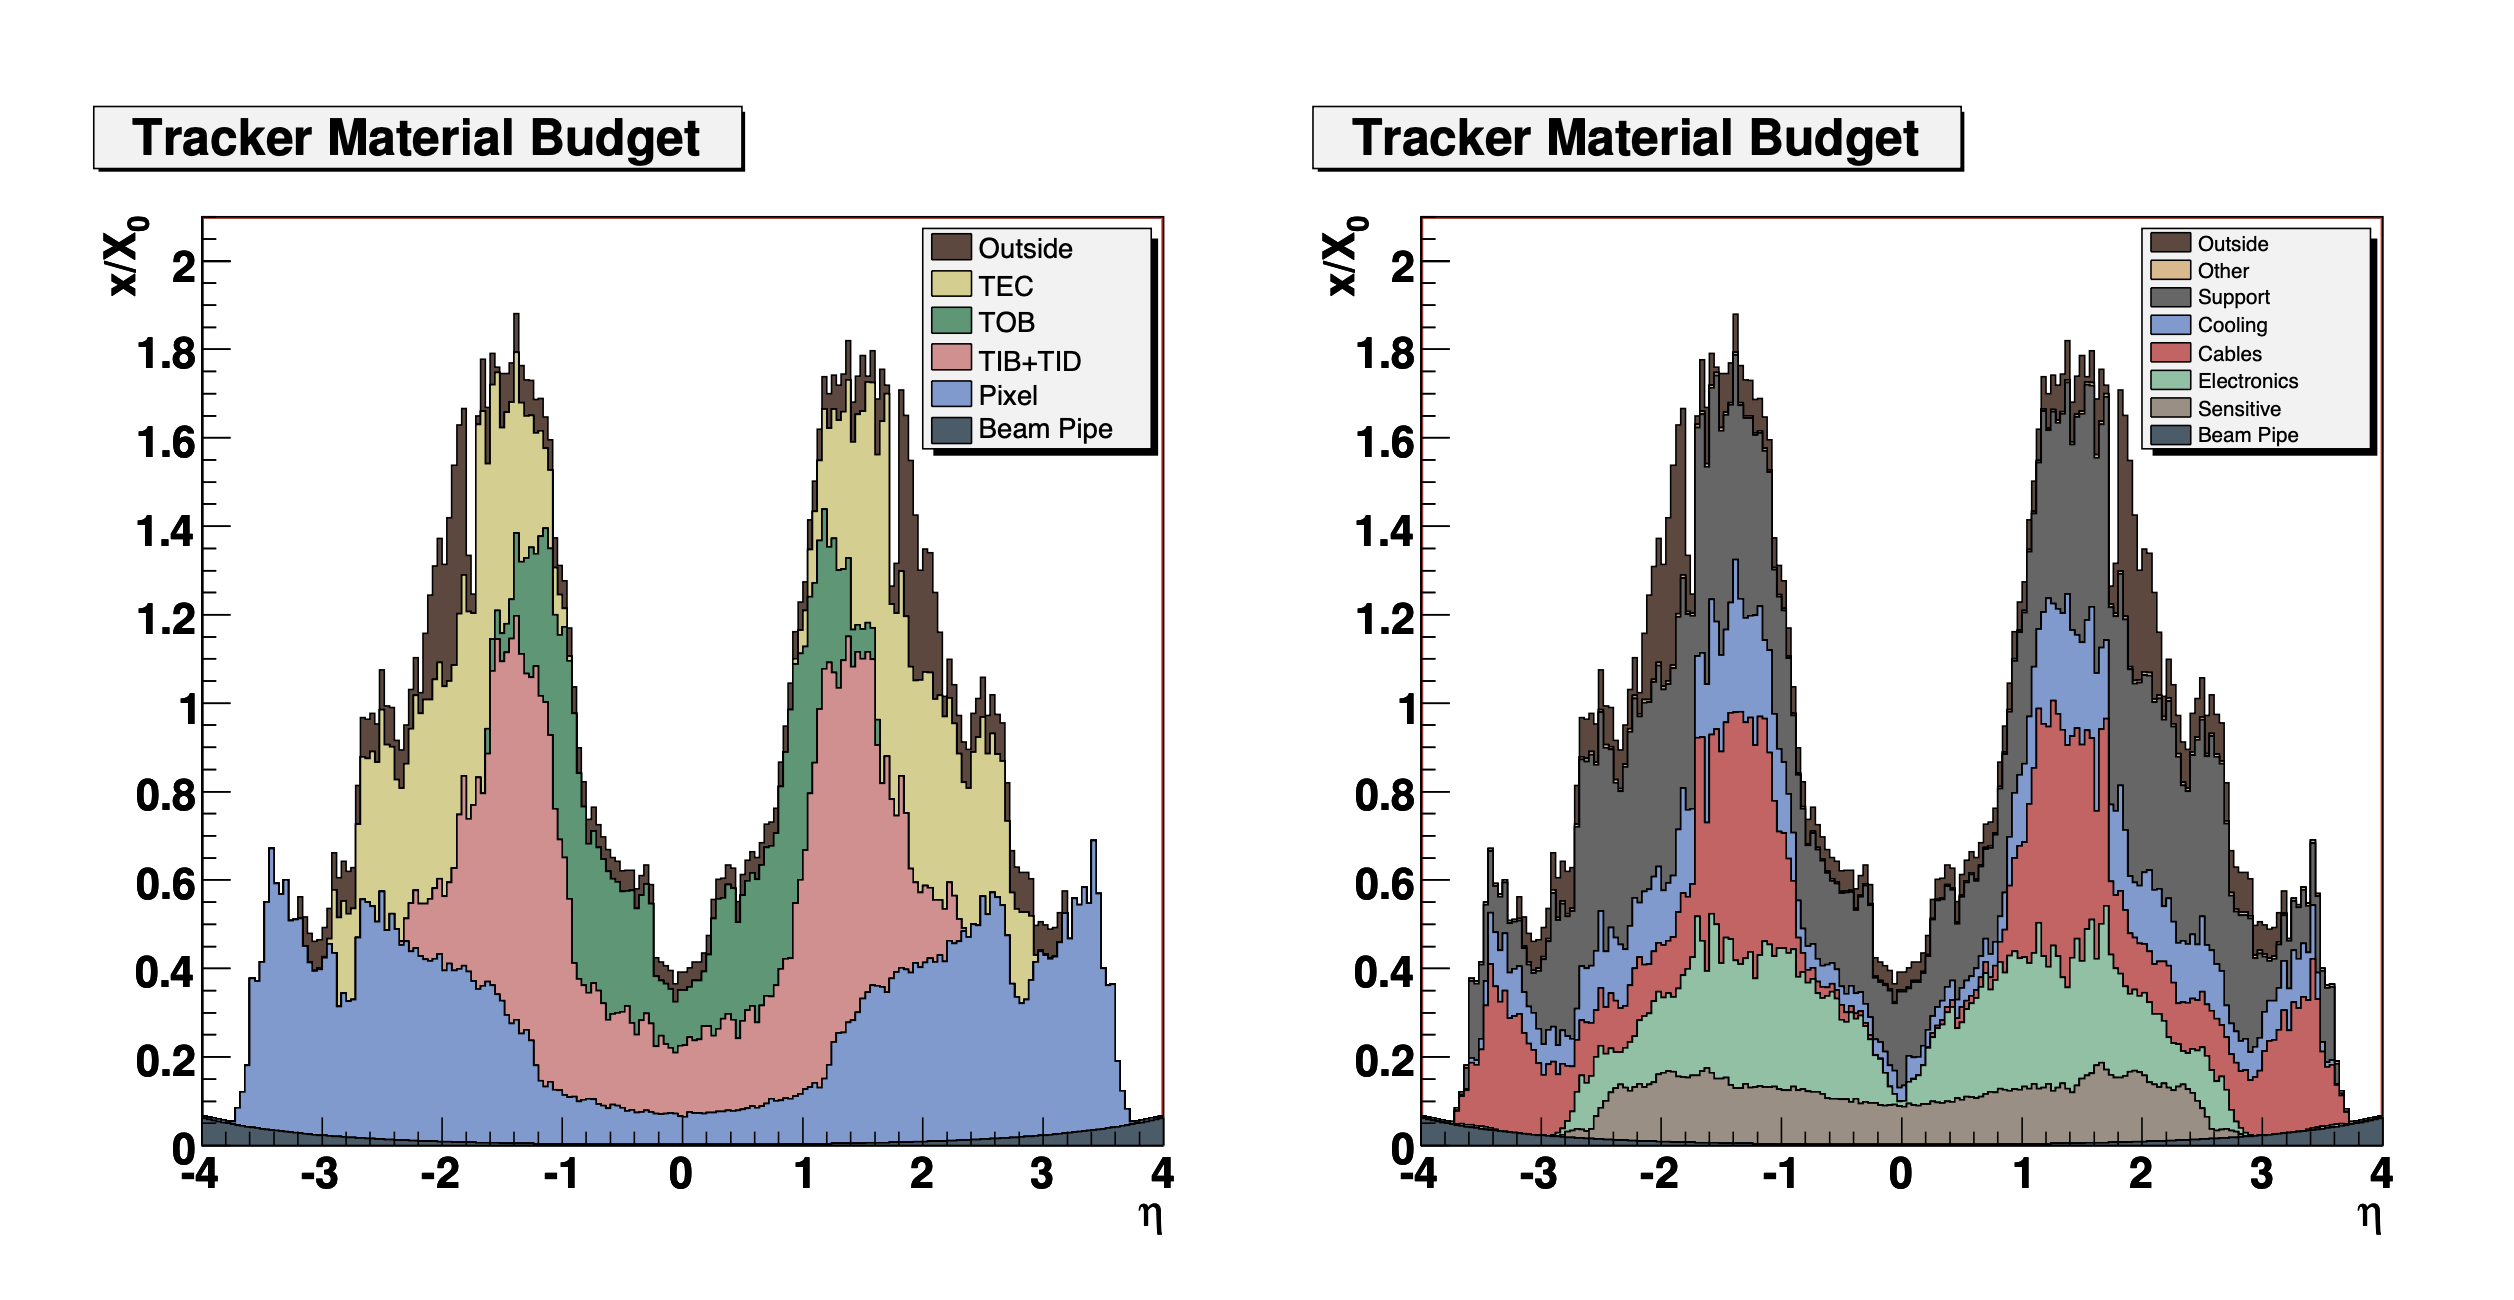
\includegraphics[width=0.98\textwidth]{chapters/CMSExperiment/sectionDetector/figures/trackerMaterial.png}
    \caption{The material thickness of the inner tracking system.}
    \label{fig:cmsexperiment:detector:trackerMaterial}
\end{figure}




% pixel
The pixel detector, shown in the center of Figure~\ref{fig:cmsexperiment:detector:tracker}, is consist of three cylindrical layers of pixel detector modules at radii of 4.4, 7.3, and 10.2~cm, totaling 66 million pixels with an area of 1~\si{\m \squared}. It is capable of producing three high precision 3D hits for each charged particle. 

% tracker
The silicon strip tracker system is immediately outside the pixel detector in the region of $20<r<116$~cm and $|z|<282$~cm. The tracker system has three parts: \acrfull{tibtid}, \acrfull{tob} and \acrfull{tec}, with a total of 9.3 million channels and 198~\si{\m \squared} active silicon area. The silicon strip modules in the barrel are laid out in cylindrical shapes with their strips parallel to the Z direction to measure $r-\phi$ coordinates. Meanwhile, those in the endcap region are in the shape of disks and place their strips in the radial direction to measure the $Z-\phi$ coordinates. In addition to the measurement of the 2D coordinates, the first two cylindrical layers of TIB and TOB, the two innermost rings of TID and TEC, as well as the fifth ring of TEC, are double-sided by placing a second micro-strip module back-to-back to the first with a stereo angle of 100~mrad. The double-sided modules can be seen in Figure~\ref{fig:cmsexperiment:detector:tracker}. This small stereo angle allows the measurement of the third spacial coordinates: $Z$ in the barrel (TIB and TOB) and $r$ on the endcap (TID and TEC). Such tracker design ensures to acquire at least 9 hits in the silicon strip tracker with at least 4 being stereo measurements. 




\begin{figure}[ht]
    \centering
    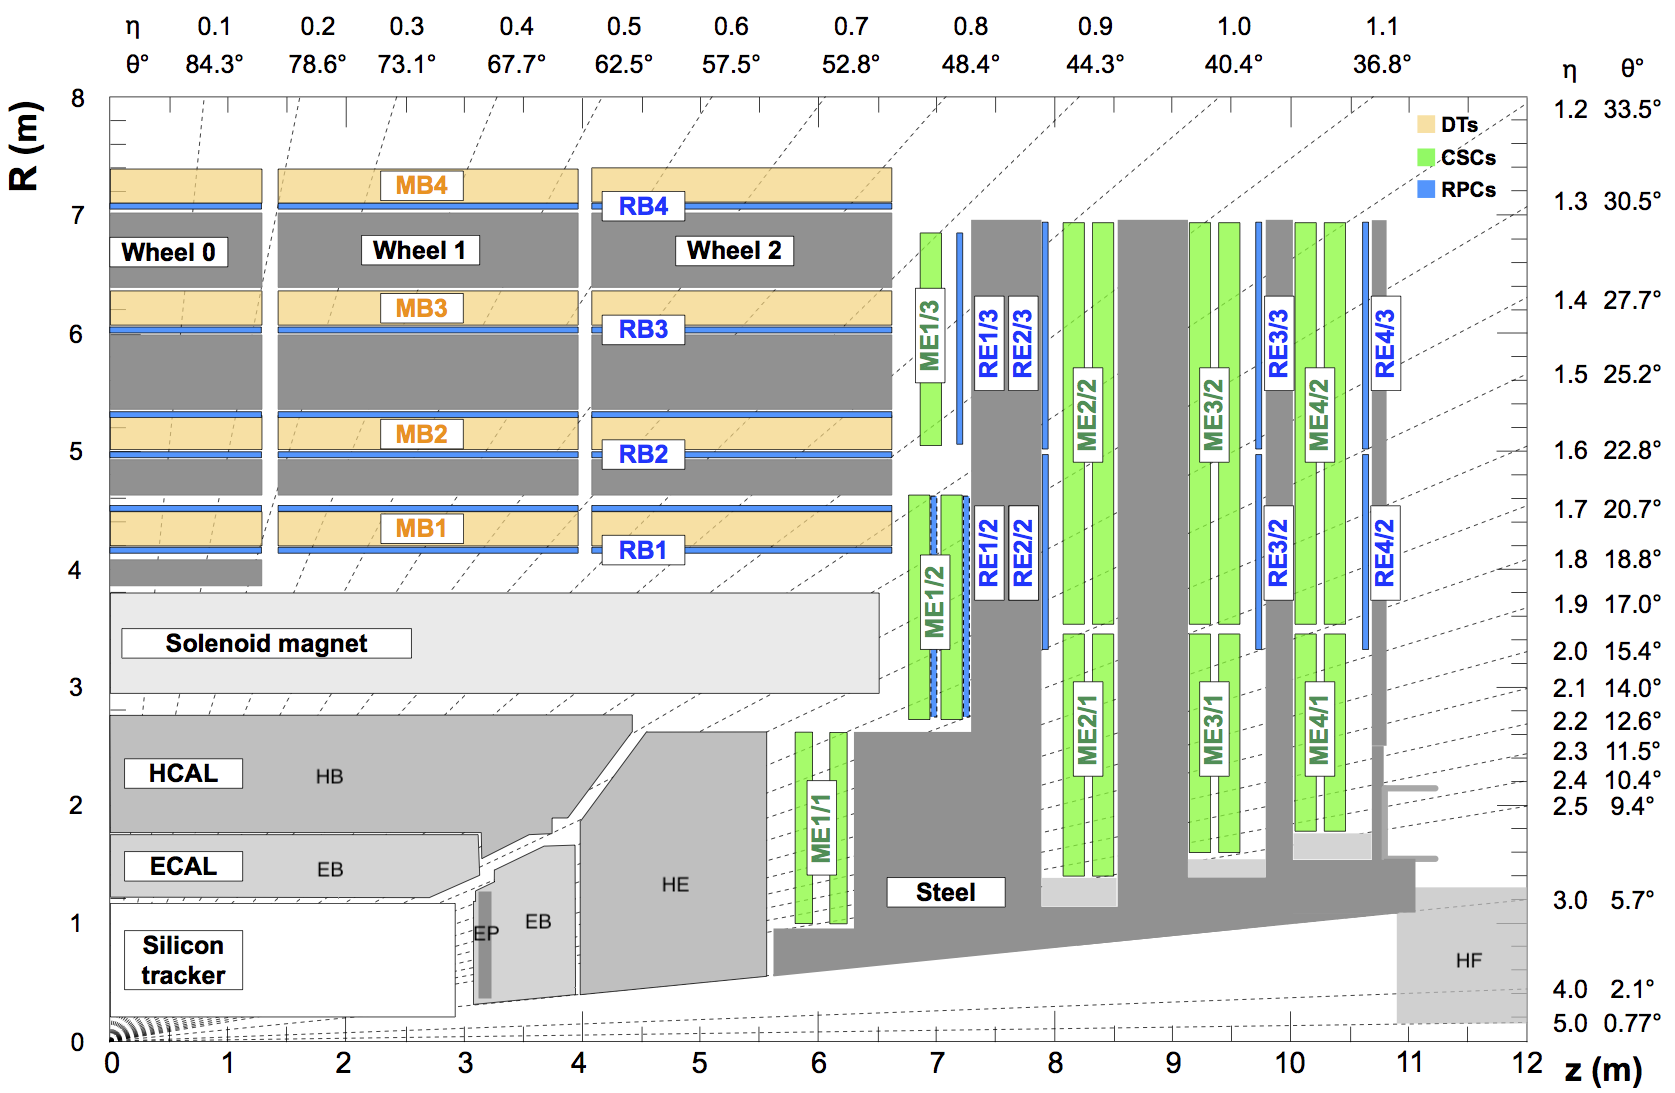
\includegraphics[width=0.98\textwidth]{chapters/CMSExperiment/sectionDetector/figures/detectorLayout.png}
    \caption{The layout of the CMS detector on the Z-r plane \cite{cms:muonChamberWebsite}. The full coverage of pseudorapidity is up to $\eta=5$. The detector includes the tracker, ECAL, HCAL, Magnets, and muon system. The details of tracker is shown in Figuge~\ref{fig:cmsexperiment:detector:tracker}. }
    \label{fig:cmsexperiment:detector:detectorLayout}
\end{figure}





\subsection{Electromagnetic Calorimeter}
%  overview
The CMS electromagnetic calorimeter (ECAL) \cite{cms:ecalTdr:CMS:1997ysd} is used to measure the energy of electromagnetic showers. As shown in Figure~\ref{fig:cmsexperiment:detector:detectorLayout}, ECAL is located immediately outside the tracking system. ECAL consists of the barrel part (EB), the endcap part (EE), and a preshower system (EP) in front of EE. EB and EE are hermetic homogeneous calorimeter made of lead tungstate crystals with \acrfull{apd} and \acrfull{vpt} as readout sensors respective. The PS is a thing sampling calorimeter with lead-silicon alternating layers to enhance the spatial resolution in the endcap region. The total ECAL material thickness is larger than 25 $\chi_0$ and about 1.1 $\lambda_I$.

% EB
The barrel part of the ECAL (EB) covers the pseudorapidity range of $|\eta|< 1.479$ and consists of 61200 crystals arranged in a $\rm 170\times360 ~ \eta - \phi$ grid, with $\rm 8.14~m^3$ of total crystal volume and 67.4~tons of weight. The crystals have a tapered shape mounted in a quasi-projective distribution, in which the crystal axis has 3-degree angle with respect to the vector from the origin to minimize chances of cracks aligned with the particle trajectories. The crystal cross-section corresponds to approximately $\Delta \eta \times \Delta\phi = 0.0174 \times 0.0174$, or $\rm 22 \times 22 ~ mm^2$ at the front face of crystal and $\rm 26\times26 ~ mm^2$ at the rear face. The crystal length is 230~mm, corresponding to 25.8~$\chi_0$.

% EE
The endcaps (EE) cover the rapidity range $1.479 < |\eta| < 3.0$ and is consist of 7324 identically shaped crystals grouped in mechanical units of 5\times 5 crystals (supercrystals, or SCs), with $\rm 2.90~m^3$ of total crystal volume and 24.0~tons of weight. The crystals are arranged in a rectangular x-y grid, with the crystals pointing at a focus 1300~mm beyond the interaction point, giving 2\textdegree-8\textdegree ~off-pointing angles. The crystals have a front face cross-section $\rm 28.62\times28.62 ~mm^2$, a rear face cross-section $\rm 30\times30~mm^2$ and a length of 220 mm, corresponding to 24.7~$\chi_0$.

% preshower
A preshower detector (EP) is placed in front of EE in $1.479 < |\eta| < 2.6$ to increase the space resolution of electromagnetic showers and better identify neutral pions $\pi^0 \to \gamma \gamma$ in the endcap. EP is a sampling calorimeter of two lead-silicon layers with a total mechanical thickness of 20~cm. On each layer, the lead radiators initiate electromagnetic showers from incoming photons and electrons, while silicon strip sensors placed after each radiator measure the deposited energy and the transverse shower profiles. The directions of silicon strips on the two layers are orthogonal to each other. The material thickness of the first and second layer are 2~$\chi_0$ and 1~$\chi_0$ respective.



\subsection{Hadronic Calorimeter}
% overview
The CMS Hadron Calorimeter \cite{cms:hcalTdrCMS:1997xji} is used to measure the energy of hadrons and determine the missing transverse energy. HCAL consists of four parts: the HCAL in the barrel region (HB), HCAL in the endcap region (HE), the forward hadronic calorimeter (HF), and a small section outside the magnetic (HO) in the barrel region. The purpose of HO is to catch the rare hadronic punch through in front of the muon system. As shown in Figure~\ref{fig:cmsexperiment:detector:detectorLayout}, HB and HE are designed right outside the ECAL, while FH is in the high pseudorapidity region outside the whole CMS endcap.

% HB, HE, HO
HB and HE are a sampling calorimeter covering $|\eta|< 1.3$ and $1.3<|\eta|< 3.0$, respectively. They use brass absorbers ($70\%$ Cu and $30\%$ Zn) and plastic scintillators for readout. HO covers the same $|\eta|< 1.3$ range as HB but uses iron as the absorber to enhance the material thickness of HB, especially in the low $\eta$ region. With HO, the total material thickness of the HCAL is about 11.8~$\lambda_I$, making sure the hadronic leakage to muon is very rare. Totally, HCAL has about 7000 scintillators channels. The spatial granularity is $\Delta \eta \times \Delta \phi = 0.087 \times 0.087$ in the HB, OB and the $1.3<|\eta|< 1.6$ part of HE. In the rest part of HE, a higher granularity of $\Delta \eta \times \Delta \phi = 0.017 \times 0.017$ is designed to increase the spatial resolution near the beam pipe.

% HF
HF is a sampling calorimeter covering $3.0 < |\eta| < 5$. It is essentially a cylindrical steel structure with fibers piecing from the back in Z direction at two different depths. Its outer radius is 130.0~cm. The front face of the calorimeter is located at 11.2~m from the interaction point. The absorber is made of steel installed perpendicular to beam pipe with a total material depth of 10~$\lambda_I$. The active material is quartz fibers (fused-silica core and polymer hard-cladding) installed in parallel with the beam pipe. When particle showers in the HF, a small part of Cherenkov light generated at the quartz fibers' surface is captured. The two different penetration depths of fibers distinguish the electromagnetic shower and the hadronic shower. The long fibers span the entire HF, while short fibers start from 22 cm behind the HF front surface and extend to the back. These fibers are bundled to form $\Delta \phi \times \Delta \eta = 0.175 \times 0.175$ towers. 


\subsection{Muon System}
% overview
The CMS muon system \cite{cms:muonChamberTdr:CMS:1997iti} is mounted in the return yoke outside the solenoid to measure the tracks of muons. The system consists of barrel detector (MB) covering $|\eta|<1.2$ and endcap detectors (ME) covering $0.9 < |\eta| < 2.4$. 

% MB RPC
The barrel detector has 250 chambers in total which hosts 250 \acrfull{dt} and 480 \acrfull{rpc}. The chambers are arranged in 4 concentric stations in the yoke, each of which is divided into 5 wheels with 12 sectors on each wheel. The two innermost stations, labeled as MB1 and MB2 in Figure~\ref{fig:cmsexperiment:detector:detectorLayout}, has two RPCs sandwiching a DT, while the 2 outermost stations, MB3 and MB4 in Figure~\ref{fig:cmsexperiment:detector:detectorLayout}, consist of a DT coupled to a layer of RPCs on the inner side. 

Each DT in MB1, MB2, and MB3 has 12 layers of drift tubes divided into 3 groups of 4 consecutive layers, called superlayers. Two superlayers with wire parallel to Z direction measure $r-\phi$ coordinates, the middle one with wire perpendicular to Z direction measures $r-z$ coordinates. DTs in MB4 only have two superlayers for measurement of $r-\phi$ coordinates. RPCs are attached to DTs to improve the responding time, which is necessary for triggers. Each RPC detector has a bakelite chamber with two 2 mm wide gaps and operates in avalanche mode biased by a high voltage. 

% ME
The endcap detectors (ME) on the two sides have 469 \acrfull{csc}s and 432 RPCs and are placed in the yokes that close the solenoid. The ME consists of 4 stations ME1-ME4. The disk of ME1 is divided into 3 concentric rings, while disks of ME2-ME4 have two rings. The details of the layout of the CSCs and RPCs in ME are shown in Figure~\ref{fig:cmsexperiment:detector:detectorLayout}. Each CSC is trapezoidal in shape and consists of 6 gas gaps. Each gap has a plane of radial cathode strips and a plane of anode wires running almost perpendicularly to the cathode strips, measuring hits with 3D coordinates.

